\documentclass[10pt]{article}
\usepackage{graphicx}
\usepackage[none]{hyphenat}
\usepackage{graphicx}
\usepackage{listings}
\usepackage[english]{babel}
\usepackage{siunitx}
\usepackage{graphicx}
\usepackage{caption} 
\usepackage{booktabs}
\usepackage{array}
\usepackage{amssymb} % for \because
\usepackage{amsmath}   % for having text in math mode
\usepackage{extarrows} % for Row operations arrows
\usepackage{listings}
\usepackage[utf8]{inputenc}
\usepackage[margin=0.5in]{geometry}
\lstset{
  frame=single,
  breaklines=true
}
\usepackage{hyperref}
  
%Following 2 lines were added to remove the blank page at the beginning
\usepackage{atbegshi}% http://ctan.org/pkg/atbegshi
\AtBeginDocument{\AtBeginShipoutNext{\AtBeginShipoutDiscard}}


%New macro definitions
\newcommand{\mydet}[1]{\ensuremath{\begin{vmatrix}#1\end{vmatrix}}}
\providecommand{\brak}[1]{\ensuremath{\left(#1\right)}}
\newcommand{\solution}{\noindent \textbf{Solution: }}
\newcommand{\myvec}[1]{\ensuremath{\begin{pmatrix}#1\end{pmatrix}}}
\providecommand{\norm}[1]{\left\lVert#1\right\rVert}
\providecommand{\abs}[1]{\left\vert#1\right\vert}
\let\vec\mathbf{}
\begin{document}

\begin{center}
\title{\textbf{STRAIGHT LINES}}
\date{\vspace{-5ex}} %Not to print date automatically
\maketitle
\end{center}

\section{11$^{th}$ Maths - Chapter 10}
This is Problem 5 from Exercise-10.4
\begin{enumerate}
\item Find perpendicular distance from the origin to the line joining the points$(\cos\theta,\sin\theta)$ and $(\cos\phi,\sin\phi)$.

\solution
Let
\begin{align}
\vec{A}=\myvec{\cos\theta\\sin\theta},\vec{B}=\myvec{\cos\phi\\sin\phi}\\
\vec{m}=\vec{B}-\vec{A}=\myvec{\cos\phi-\cos\theta\\\sin\phi-\sin\theta}\\
\end{align}
The normal vector is,
\begin{align}
\vec{n}&=\myvec{0&1\\-1&0}\myvec{\cos\phi-\cos\theta\\\sin\phi-\sin\theta}=\myvec{\sin\phi-\sin\theta\\\cos\theta-\cos\phi}\\
\norm{\vec{n}}&=\sqrt{\brak{\sin\phi-\sin\theta}^2+\brak{\cos\theta-\cos\phi}^2}\\
&=\sqrt{2-2\brak{\sin\phi\sin\theta+\cos\phi\cos\theta}}\\
&=\sqrt{2-2\brak{\cos\brak{\phi-\theta}}}\\
&=\sqrt{2\brak{1-\cos\brak{\phi-\theta}}}\\
&=\sqrt{2\brak{2\sin^2\brak{\frac{\phi-\theta}{2}}}}\\
\implies\norm{\vec{n}}&=2\sin\brak{\frac{\phi-\theta}{2}}
\end{align}
The line equation is,
\begin{align}
\vec{n}^\top\brak{\vec{x}-\vec{A}}&=0\\
\implies\myvec{\sin\phi-\sin\theta&\cos\theta-\cos\phi}\brak{\vec{x}-\myvec{\cos\theta\\\sin\theta}}&=0\\
\implies\myvec{\sin\phi-\sin\theta&\cos\theta-\cos\phi}\vec{x}&=\myvec{\sin\phi-\sin\theta&\cos\theta-\cos\phi}\myvec{\cos\theta\\\sin\theta}\\
&=\brak{\sin\phi-\sin\theta}\cos\theta+\brak{\cos\theta-\cos\phi}\sin\theta\\
&=\sin\phi\cos\theta-\sin\theta\cos\theta+\sin\theta\cos\theta-\sin\theta\cos\phi\\
\implies\myvec{\sin\phi-\sin\theta&\cos\theta-\cos\phi}\vec{x}&=\sin\brak{\phi-\theta}
\label{eq:1}
\end{align}
from \eqref{eq:1}
\begin{align}
c=\sin\brak{\phi-\theta}
\end{align}
The perpendicular distance from the origin to the line is
\begin{align}
d&=\frac{\abs{c}}{\norm{\vec{n}}}\\
\implies d&=\frac{\sin\brak{\phi-\theta}}{2\sin\brak{\frac{\phi-\theta}{2}}}
\end{align}
\begin{figure}[!h]
	\begin{center}
		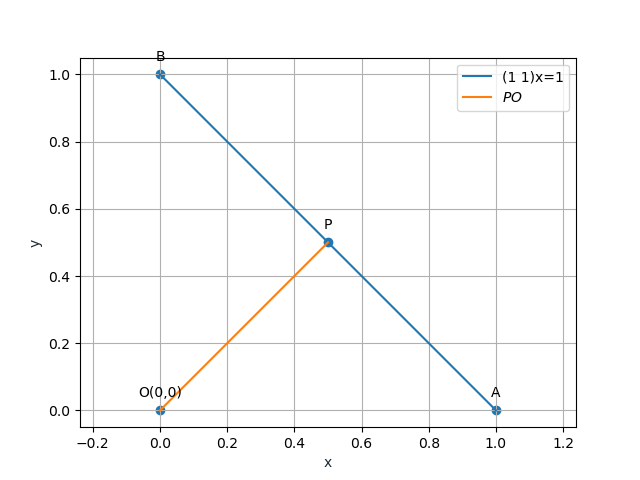
\includegraphics[width=\columnwidth]{./figs/fig.png}
	\end{center}
\caption{}
\label{fig:Fig1}
\end{figure}

\end{enumerate}
\end{document}
